\documentclass[11pt, letterpaper]{article}
%\usepackage[showframe]{geometry}
%\usepackage{layout}

\setlength{\voffset}{-1.1in}
\setlength{\headsep}{5pt}
\setlength{\footskip}{20pt}
\setlength{\textheight}{660pt}

\usepackage{verbatim} % for comments
\usepackage{mathtools}
\usepackage{graphicx}
\usepackage{caption}
\usepackage{subcaption}
\usepackage{float}

\title{\textbf{2D Poisson}}
\author{Ramya Rao Basava\\
Department of Computer Science\\
University of British Columbia, Vancouver}
\date{}

\begin{document}%\layout
\maketitle

\section{Problem Statement}
Consider the 2D Poisson problem with essential boundary conditions as given
below:
\begin{align*}
\Delta u (x,y) &= (x^2+y^2)e^{xy} &\text{in} \quad \Omega = \{(x,y) \vert 0 < x < 1,0 < y < 1\} \\
u (x,y) &= e^{xy} \quad &\text{on }  \partial\Omega = \{(x,y) \vert x=0,1 \text{ and } y=0,1\}
\end{align*}

The analytical solution to the problem is $u (x,y) = e^{xy}$.

\section{Numerical Analysis}

The domain is discretized using $10\times10$ source points and  $40\times40$ collocation points which do not overlap as shown in Figure \ref{fig1}. 

\begin{figure}[H]
\centering
\begin{subfigure}{.5\textwidth}
  \centering
  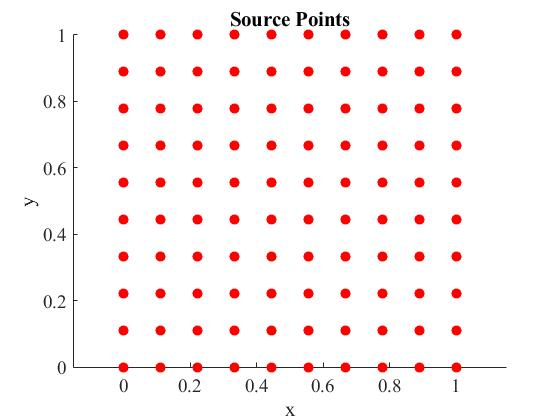
\includegraphics[width=0.97\linewidth]{images/5.jpg}
  \caption{Source points}
  \label{fig1-1}
\end{subfigure}%
\begin{subfigure}{.5\textwidth}
  \centering
  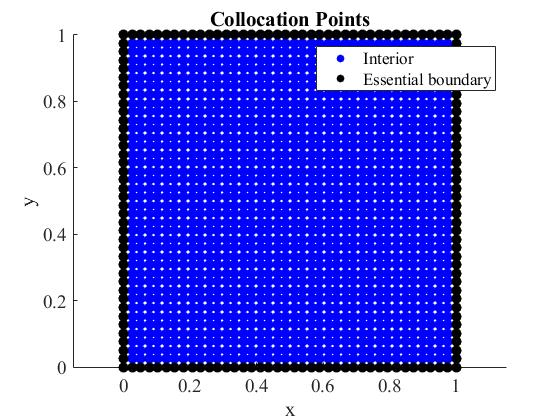
\includegraphics[width=0.97\linewidth]{images/6.jpg}
  \caption{Collocation points}
  \label{fig1-2}
\end{subfigure}
\caption{Domain discretization}
\label{fig1}
\end{figure}

The weight on the essential boundary is taken to be $\sqrt{\alpha^g}=N_S$, where $N_S$ is the number of source points. The numerical and analytical solutions in the 2D domain are compared in Figure \ref{fig2}.

\begin{figure}[H]
\centering
\begin{subfigure}{.5\textwidth}
  \centering
  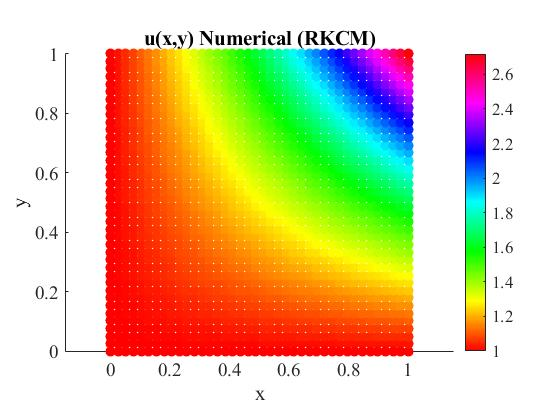
\includegraphics[width=0.97\linewidth]{images/1.jpg}
  \caption{Numerical}
  \label{fig2-1}
\end{subfigure}%
\begin{subfigure}{.5\textwidth}
  \centering
  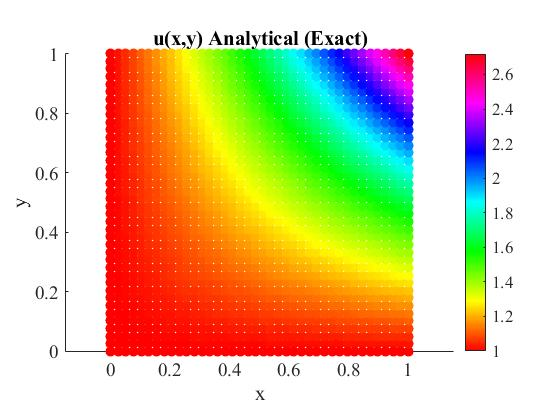
\includegraphics[width=0.97\linewidth]{images/2.jpg}
  \caption{Analytical}
  \label{fig2-2}
\end{subfigure}
\caption{Comparison of numerical and analytical solution in 2D domain}
\label{fig2}
\end{figure}

Additionally, the numerical solution using RKCM obtained along the diagonal line passing through the points $(0,0)$ and $(1,1)$ is plotted in Figure \ref{fig3} and compared with the analytical solution. The error between the two solutions along this diagonal line is also plotted. 

\begin{figure}[H]
\centering
\begin{subfigure}{.5\textwidth}
  \centering
  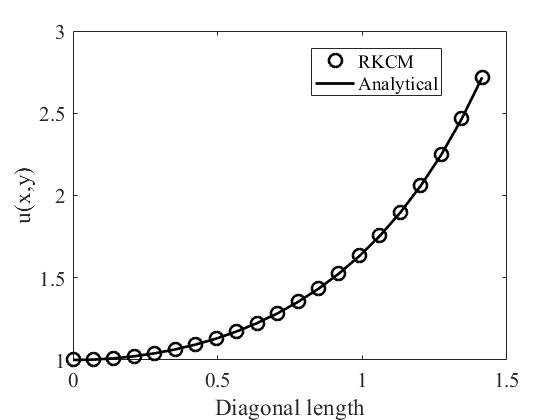
\includegraphics[width=0.97\linewidth]{images/3.jpg}
  \caption{Solution comparison}
  \label{fig3-1}
\end{subfigure}%
\begin{subfigure}{.5\textwidth}
  \centering
  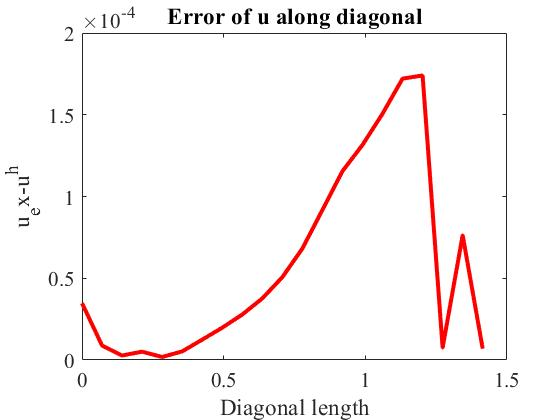
\includegraphics[width=0.97\linewidth]{images/4.jpg}
  \caption{Error}
  \label{fig3-2}
\end{subfigure}
\caption{Comparison of numerical and analytical solution along the diagonal line}
\label{fig3}
\end{figure}



It can be seen that the numerical RKCM result is very close to the analytical solution. 





\end{document}













